The current developing status of the country means the cost is the primary factor determining how energy is sourced. Tanzania contains a wide range of biomes, where fundamental factors such as humidity, accessibility and existing infrastructure affect how cheap energy can be supplied. Where "average walk to water" statistics exist, conventional RE motivation does not apply. However, RE still plays a significant role in providing localised power to remote areas. 

Solar panels have the advantage of being cheap, requiring little infrastructure and do not need any fuel to run. This makes them perfect for powering low-power electronics increasing the quality of life of the average Tanzanian.

The GPD per capita of Tanzania shows stable exponential growth. Extrapolating this growth will introduce more energy-intensive sectors such as transport and industry. Hence will increase the energy demand of the country. While renewable energy is cheap on small scales, it does not scale well. Hence, the country will likely look to other cheaper forms of energy to power the country.  


\begin{figure}
    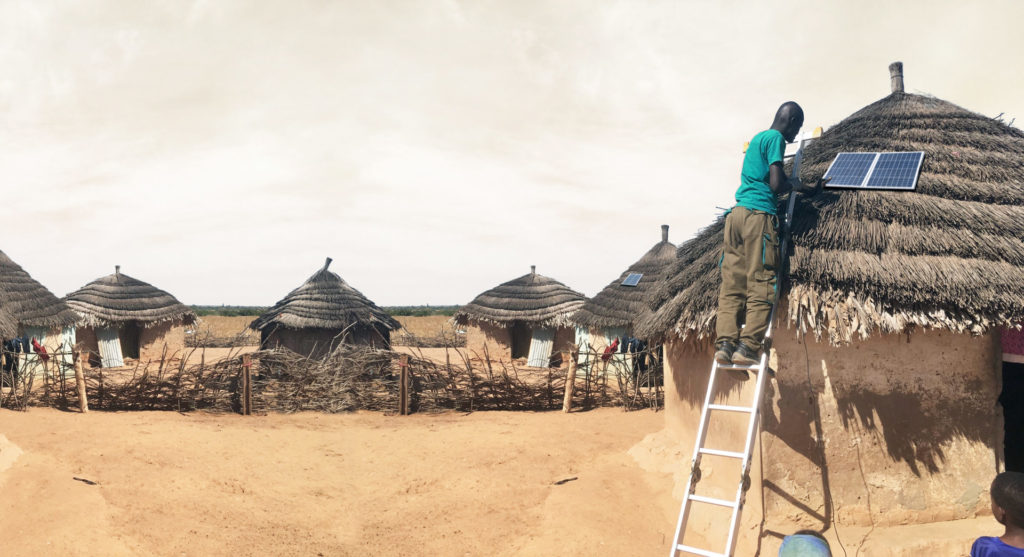
\includegraphics[width=0.7\textwidth]{IMG/solar-roof.jpg}
    \caption{Solar panels being fitted to a rondavel \cite{Cullmann2020Feb}}
    \end{figure}\label{fig:4_Review_3}
    

